\documentclass{article}
\usepackage[utf8]{inputenc}
\usepackage[T1]{fontenc}
\usepackage[english]{babel}
\setlength{\parindent}{0pt}
\usepackage{hyperref}
\hypersetup{
    colorlinks=true,
    linkcolor=blue,
    filecolor=magenta,      
    urlcolor=cyan}
\usepackage{graphicx}
\graphicspath{ {./pic/} }
\usepackage{multicol}
\usepackage{lscape}

\usepackage{fourier,amssymb,microtype,amsmath,gensymb}
\newcommand{\R}{\mathbb{R}}
\usepackage{mdframed,caption,xcolor}
\usepackage{tikz,tkz-euclide}

\title{Seminar 8. Mixed Strategies and Repeated Games}
\author{Xiaoguang Ling \\  \href{xiaoguang.ling@econ.uio.no}{xiaoguang.ling@econ.uio.no}}
\date{\today}

\begin{document}

\maketitle

%%%%%%%%%%%%%%%%%%%%%%%%%%%%%%%%%%%%%%%%%%%%%%%%%%%%%%%%%%%%%%%%%%%%%%%%%%%%%%%%%%%%%%%%%%%%%%

\section{Problem 1 - BR and UD} 

For each of the statements, if true, try to explain why, and if false, provide a
counter-example.

\bigskip

(a) In a finite normal-form game, if a pure strategy of a
player is \textbf{not a best response} to any belief that the player has about the strategies played by his opponents, then this pure strategy is strictly dominated by another \textbf{pure} strategy.\\

\medskip

False. It may be dominated by mixed strategies.
Consider:

\begin{center}
\captionof{table}{BR and UD for a 2-player normal form game}
\label{tab:brud}
\begin{tabular}{cc|c|c|}
  & \multicolumn{1}{c}{} & \multicolumn{2}{c}{$P2$}  \\
  & \multicolumn{1}{c}{} & \multicolumn{1}{c}{$d$} & \multicolumn{1}{c}{$e$} \\\cline{3-4}
            & $a$ & $(3,-)$ & $(0,-)$ \\   \cline{3-4}  
   $P1$ & $b$ & $(0,-)$ & $(3,-)$ \\   \cline{3-4}
            & $c$ & $(1,-)$ & $(1,-)$ \\   \cline{3-4}

\end{tabular}
\end{center}

The pure strategy $c$ is not a best response to any belief about $d$ and $e$.

\smallskip

\begin{mdframed}[backgroundcolor=blue!20,linecolor=white]
The correct statement is (Watson pp.58):

\begin{itemize}
\item In a finite two-player game,$B_1 = UD_1$ and $B_2 = UD_2$
\item For finite games with more than 2 players, read Watson Appendix B (pp.423) if you're interested.
\end{itemize}

And Dominance is defined as:

\textbf{Dominance}(Watson pp.50): A pure strategy $s_i$ of player $i$ is dominated if there is a strategy (\textbf{pure or mixed}) $\sigma_i \in \Delta S_i$ such that $u_i(\sigma_i , s_{−i}) > u_i (s_i , s_{−i})$, for all strategy profiles $s_{−i} \in S_{−i}$ of the other players.

\medskip

A more general question can be: find $B_i$ for any possible belief.
(don't forget mixed strategies)

\medskip

Procedure for calculating $B_i$ (also $UD_i$) for two-player matrix games:

\begin{enumerate}
\item Look for strategies that are best responses to the simplest beliefs -- those beliefs that put all probability on just one of the other player's strategies.These best responses are obviously in the set $B_i$ so they are also in $UD_i$ .
\item Look for strategies that are dominated by other pure strategies; these dominated strategies are not in $UD_i$ and thus they are also not in $B_i$.
\item Test each remaining strategy to see if it is dominated by a \textbf{mixed strategy}. This final step is the most difficult, but if you are lucky, then you will rarely have to perform it.

\end{enumerate}

Let's look for $BR_1$ (which is also $UD_1$) in Table \ref{tab:brud}.

\begin{enumerate}
\item $BR_1(d)=a$, $BR_1(e)=b$, thus ${a,b}$ are obviously in the set $B_1$ (and $UD_1$).
\item ${c}$ is not dominated by any other pure strategies.
\item Can ${c}$ be dominated by a mixed strategy of $a,b$? Yes (and it must be, accoding to Watson pp.58), for example, a mix strategy between ${a,b}$ with probability $(0.5,0.5)$ yeilds expected payoff $(1.5,1.5)$
\end{enumerate}

More precisely, let $q$ be the probability assigned to $a$ and $1-q$ the probability assigned to $b$.If ${c}$ is dominated by a mixed strategy of $a$ and $b$, we must have:

$$q\times 3 + (1-q)\times 0 > 1 \Rightarrow q > \tfrac13 $$
$$q\times 0 + (1-q)\times 3 >1 \Rightarrow p < \tfrac23 $$

That is, if $q\in (\tfrac13,\tfrac23)$, ${c}$ is dominated by a mixed strategy of $a$ and $b$.

\end{mdframed}


%
(b) In a finite normal-form game, if a pure strategy of a
player is not a best response to any belief that the player has about the strategies played by his opponents, then this pure strategy is strictly dominated by some \textbf{mixed} strategy.

\medskip

True for a two-player game. In a finite two-player game,$B_1 = UD_1$ and $B_2 = UD_2$. A non-BR must not be UD either, thus it must be dominated by some strategy (recall: a so called pure strategy is simply a mixed strategy with belief like $(1,0,\cdots)$).


\begin{mdframed}[backgroundcolor=blue!20,linecolor=white]
It is outside the scope of this course to provide a formal proof of this result. In particular, in games with three or more player, the result requires that a player might have correlated beliefs about the strategies played by his opponents.

\smallskip

Read Watson Appendix B (pp.423) if you're interested in games with more than 2 players.
\end{mdframed}

%%%%%%%%%%%%%%%%%%%%%%%%%%%%%%%%%%%%%%%%%%%%%%%%%%%%%%%%%%%%%%%%%%%%%%%%%%%%%%%%%%%%%%%%%%%%%%
\newpage
\section{Problem 2 - Penalty kick} 

(Jehle and Reny pp.367, Problem 7.13)

Consider the penalty kick in soccer. There are two players, the goalie and the striker. 
\begin{itemize}
\item The striker has two strategies: kick to the goalie's right ($R$) or to the goalie's left ($L$). 
\item The goalie has two strategies: move left ($L$) or move right ($R$). 
\end{itemize}

Let $\alpha$ be the probability that the kick is stopped when both choose
L, and let $\beta$ be the probability that the kick is stopped when both choose $R$. 

Assume that $0 < \alpha < \beta < 1$. Consequently, the striker is more skilled at kicking to the goalie's left. The payoff matrix is as follows.

\begin{center}
{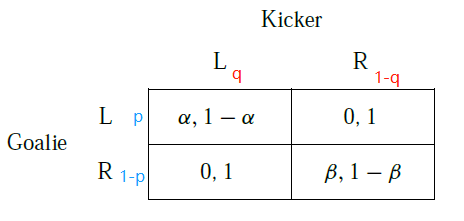
\includegraphics[width=0.5\textwidth]{8.q7_13}
\label{fig:q7_13}
\vspace{2mm}}
\end{center}


\subsection*{(a) Before analysing this game, informally answer the following questions.}

\begin{itemize}
\item Would you expect a striker who is more skilled at kicking to the goalie's left than to his right, to score more often when he kicks to the goalie's left?

\begin{mdframed}[backgroundcolor=blue!20,linecolor=white]
Will there be any dominated strategy in the end? No. The goalie knows clearly about the kicker's skill, and will pay more attention to the left side too.


\end{mdframed}


\item If a striker's ability to score when kicking to the goalie's left rises (i.e. $\alpha$ decreases) how will this affect the percentage of times the striker scores when he chooses to kick to the goalie's left? Will it affect his scoring percentage when he kicks right?

\begin{mdframed}[backgroundcolor=blue!20,linecolor=white]
Improvement on kicking skills is a good thing for the kicker anyway. But the goalie is always watching!
\end{mdframed}

\end{itemize}




\subsection*{(b) Find the unique Nash equilibrium.}

\begin{mdframed}[backgroundcolor=blue!20,linecolor=white]
Obviously $L$ and $R$ are not dominated by each other (as pure strategies) for the two players. Now consider the 
mixed strategy case.
\end{mdframed}

Let $p$ be the probability that the Goalie moves $L$ and $1-p$ the probability that the Golie moves $R$, and let $q$ be the probability that the Striker kicks $L$ and $1-q$ the probability that the Striker kicks $R$. This yields the following payoffs:

\newpage

For Goalie:
\begin{itemize}
\item If moves $L$: $E(U^G_L)= q \alpha + (1-q) \times 0 = q \alpha$.
\item If moves $R$: $E(U^G_R)=q \times 0 + (1-q) \beta =(1-q) \beta$.
\end{itemize}

For Kicker
\begin{itemize}
\item If kicks $L$: $E(U^K_L) = p (1-\alpha) + (1-p)\times 1 = 1 - p\alpha$.
\item If kicks $R$: $E(U^K_R) = p\times 1 + (1-p)(1-\beta) = p + 1 - p - \beta + p\beta = 1 - (1-p)\beta$.
\end{itemize}

\begin{mdframed}[backgroundcolor=blue!20,linecolor=white]
To make the mixed strategy rational, the players must be indifferent bweteen $L$ and $R$. Otherwise one strategy must be
dominated by another.
\end{mdframed}


$$E(U^G_L) = E(U^G_R) \Rightarrow  q(\alpha+\beta) = \beta \Rightarrow q=\frac{\beta}{\alpha+\beta}$$
 
$$E(U^K_L) = E(U^K_R) \Rightarrow 1- p\alpha = 1-(1-p)\beta \Rightarrow p = \frac{\beta}{\alpha+\beta}$$

 
NE: both players choose $L$ with probability $\tfrac{\beta}{\alpha + \beta}$, and $R$ with probability $\tfrac{\alpha}{\alpha + \beta}$. 

   
\subsection*{(c) Answer again the questions in part (a).}

 Based upon this, would it be wise to judge a striker's relative scoring ability in kicking left versus right by comparing the fraction of times he scores when he kicks right versus the fraction of times he scores when he kicks left?

\medskip

\textbf{(i) Will the kicker score more often at left?}

\medskip

$Pr(score|L) = Pr($Goalie moves to R$) + Pr($Goalie moves to L \&  failed to stop it$)$

\medskip

Thus, 
\begin{align*}
Pr(score|L) &= (1-p) + p \times (1-\alpha) \\
&= (1-\tfrac{\beta}{\alpha + \beta}) + \tfrac{\beta}{\alpha + \beta} (1-\alpha) \\
&= 1- \tfrac{\alpha \beta }{\alpha + \beta} 
\end{align*}


$Pr(score|R) = Pr($Goalie moves to L$) + Pr($Goalie moves to R \&  failed to stop it$)$

\medskip

Thus, 

\begin{align*}
Pr(score|R) &= p + (1-p)\times (1-\beta)  \\
&= \tfrac{\beta}{\alpha + \beta} + (1-\tfrac{\beta}{\alpha + \beta}) (1-\beta) \\
&=  1- \tfrac{\alpha \beta }{\alpha + \beta}
\end{align*}

In the Nash equilibrium, the scoring probability is the same for both $L$ and $R$.


\begin{mdframed}[backgroundcolor=blue!20,linecolor=white]
The Kicker is better at Left, but the goalie is aware of that and goes more often to the Left.

\end{mdframed}


\textbf{(ii) If the striker's ability to score when kicking left rises ($\alpha$ decreases), how will this affect $Pr(score|L)$ and $Pr(score|R)$}

\medskip

We already know $$Pr(score|L) = Pr(score|R)= 1- \tfrac{\alpha \beta }{\alpha + \beta} =  1- \tfrac{\beta }{1 + \frac{\beta}{\alpha}}$$

When $\alpha$ decreases, the scoring probabilities for $L$ and $R$ are increased, but $Pr(score|L) = Pr(score|R)$ still holds for the NE.

\medskip

Therefore, it is not wise to judge a striker's relative scoring ability in kicking left versus right by comparing the fraction of times he scores when he kicks right or left.


\subsection*{(d) Show that knowing the $Pr(score|$both L$)$ and $Pr(score|$both R$)$ would permit you to correctly deduce the player's scoring ability when kicking left and right.}

The probability of scoring if both choose $L$ is $1 - \alpha$, and the probability of scoring if both choose $R$ is $1 - \beta$. 


Once you konw the relation between $1 - \alpha$ and $1 - \beta$, you also know the relation between $\alpha$ and $\beta $. For example: $1 - \alpha > 1 - \beta \iff \alpha <  \beta $, Kicker is better at Left.


\subsection*{(e) Could you correctly deduce the player's scoring ability kicking left versus right if you only had access to the striker's choice? If not, what can be deduced?}

The striker's choice at NE is $(\tfrac{\beta}{\alpha + \beta},\tfrac{\alpha}{\alpha + \beta})$.
Once you know relation between $\tfrac{\beta}{\alpha + \beta}$ and $\tfrac{\alpha}{\alpha + \beta}$, you also know the relation between $\alpha$ and $\beta $.


\subsection*{(f) Could you correctly deduce the player's scoring ability when kicking left versus right if you only had access to the goalie's choice? If not, what can be deduced?}

The same as (e)


%%%%%%%%%%%%%%%%%%%%%%%%%%%%%%%%%%%%%%%%%%%%%%%%%%%%%%%%%%%%%%%%%%%%%%%%%%%%%%%%%%%%%%%%%%%%%%
\newpage

\section{Problem 3 - Reporting a crime}

A crime is observed by a group of $n$ people. Each person would like the police to be informed
but prefers that someone else make the phone call. Specifically, suppose that each person
attaches the value $v$ to the police being informed and bears the cost $c$ if she makes the
phone call, where $v > c > 0$.

\subsection*{(a) Model this situation as normal form game.}  


 Players: $N = \{1, \dots , n \}$ \\ 
 Strategy set for each player: $\{A, I \}$, where $A$: action and $I$: inaction \\ 
 Payoff function: 

\begin{itemize}
\item $0$ if self and others choose $I$; 
\item $v-c$ if self choose $A$; 
\item $v$ is self choose $I$ and some other choose $A$.
\end{itemize}




%
\subsection*{(b) Find the set of pure strategy Nash equilibria. } 

There are $n$ different asymmetric pure strategy Nash equilibria where exactly one chooses $A$:

$$(A,I,I,\cdots,I)$$
$$(I,A,I,\cdots,I)$$
$$\cdots$$
$$(I,I,I,\cdots,A)$$

\begin{mdframed}[backgroundcolor=blue!20,linecolor=white]

Check the payoff to see if there is any incentive to deviate from the NE. For example, the payoff for
$(A,I,I,\cdots,I)$ is $(v-c,v,v,\cdots,v)$.

\begin{itemize}
\item Will player 1 deviate (from A to I)? No, deviation leads to a lower payoff (from $v-c$ to $0$)
\item Will any other player deviate (from I to A)? No, deviation leads to a lower payoff ($v$ to $v-c$)
\end{itemize}

Using the same method, it's clear that "nobody acts" $(I,I,I,\cdots,I)$ and "more than 1 act" $(I,A,A,\cdots,I)$ are
unstable.
\end{mdframed}


\subsection*{(c) Find the symmetric mixed strategy Nash equilibrium.}

\begin{mdframed}[backgroundcolor=blue!20,linecolor=white]
If there is a dominated strategy, the player will assgin 0 probability to it. Therefore:
\end{mdframed}

In a mixed strategy mixed strategy Nash equilibrium, the players must be \textbf{indifferent between $A$ and $I$}.
\begin{align*}
& U^i_A = v-c \\  
&E(U^i_I) = 0 \times Pr(\text{no one else acts}) + v \times  Pr(\text{at least one else acts}) \\
&= 0 + v \times [1- Pr(\text{no one else acts})]
\end{align*}
$$U^i_A = E(U^i_I) \Rightarrow v-c = v [1- Pr(\text{no one else acts})]\Rightarrow Pr(\text{no one else acts}) = \frac{c}{v}$$
If we denote the probability of choosing $A$ by $p$, choosing $I$ by $1-p$ (note by "symmetric", we assume all individuals are identical and independent), 
this implies:

$$Pr(\text{no one else acts}) = (1-p)^{n-1} \Rightarrow \frac{c}{v}= (1-p)^{n-1} \Rightarrow  p = 1 - \left( \tfrac{c}{v} \right)^\frac1{n-1}$$ 


\subsection*{(d) In the symmetric mixed strategy NE, how does the \\ $Pr(\text{the police  will  be  called})$ vary with the number of people $n$?}  

\begin{align*}
Pr(\text{the police  will  be  called}) &= 1 - Pr(\text{nobody acts})  \\
&= 1- (1-p)^n \\
&= 1- \left( \tfrac{c}{v} \right)^\frac n{n-1} \\
&= 1- \left( \tfrac{c}{v} \right)^\frac 1{1-\tfrac 1n}
\end{align*}

\begin{itemize}
\item $\tfrac{c}{v} \in (0,1)$
\item $\frac 1{1-\tfrac 1n} > 1$, and decreasing in $n$.
\end{itemize}

$\left( \tfrac{c}{v} \right)^\frac 1{1-\tfrac 1n}$ is increasing in $n$, thus $Pr(\text{the police  will be called})$ is decreasing in $n$.

\begin{mdframed}[backgroundcolor=blue!20,linecolor=white]
This is one explanation of the so-called ``bystander effect''.
\end{mdframed}

\begin{mdframed}[backgroundcolor=yellow!20,linecolor=white]

Examples can be helpful to avoid mistakes. If there are only 2 people, $1-\left( \tfrac{c}{v} \right)^\frac 1{1-\tfrac 1 2} =1- \left( \tfrac{c}{v} \right)^2$; if there are infinite people,  $1- \left( \tfrac{c}{v} \right)^\frac 1{1-\tfrac 1 2} =1- \tfrac{c}{v}$.

\smallskip
You can also use derivatives to show monotonicity.
\end{mdframed}



%%%%%%%%%%%%%%%%%%%%%%%%%%%%%%%%%%%%%%%%%%%%%%%%%%%%%%%%%%%%%%%%%%%%%%%%%%%%%%%%%%%%%%%%%%%%%%

\section{Problem 4 - Finitely repeated game}

(Watson Exercise pp.308 Q22.4)

If its stage game has exactly one Nash equilibrium, how many subgame
perfect equilibria does a two-period, repeated game have? Explain. 

\smallskip

Would your answer change if there were $T$ periods, where $T$ is any finite integer?

\bigskip


\begin{itemize}
\item For a two-period game: In period 2, subgame perfection requires play of the \textbf{only} NE
of the stage game. Thus, the only subgame perfect equilibrium the stage NE in both periods. 

\item For any finite T, the logic from the two-period case applies, and the answer does not
change.

\end{itemize}

\begin{mdframed}[backgroundcolor=blue!20,linecolor=white]
As there is only one NE of the stage game,
selection of the NE to be played in period 2 cannot influence
incentives in period 1.

\medskip 

If there are more than one NE in period 2, 
the player may threat the opponent by choosing which NE to take in period 2.

\end{mdframed}


%%%%%%%%%%%%%%%%%%%%%%%%%%%%%%%%%%%%%%%%%%%%%%%%%%%%%%%%%%%%%%%%%%%%%%%%%%%%%%%%%%%%%%%%%%%%%%

\section{Problem 5 - Infinitely repeated game}

Consider the following normal form game.

\begin{center}
\captionof{table}{Infinitely repeated game}
\label{tab:infi}
\begin{tabular}{cc|c|c|c|}
  & \multicolumn{1}{c}{} & \multicolumn{3}{c}{$P2$}  \\
  & \multicolumn{1}{c}{} & \multicolumn{1}{c}{$L$} & \multicolumn{1}{c}{$C$} & \multicolumn{1}{c}{$R$} \\\cline{3-5}
            & $U$ & $(1,1)$ & $(4,0)$  & $(5,0)$ \\   \cline{3-5}  
      $P1$  & $M$ & $(0,4)$ & $(3,3)$  & $(6,2)$ \\   \cline{3-5}
            & $D$ & $(0,5)$ & $(2,6)$  & $(5,5)$ \\   \cline{3-5}

\end{tabular}
\end{center}

Assume now that this game is repeated \textbf{infinitely} many times. Assume furthermore that the players in each round can observe choices made in earlier rounds and that their payoff is the sum of payoffs discounted by the discount factor   $\delta$ (where $0 < \delta < 1$). Show that there exists a subgame perfect Nash equilibrium leading to the outcome path
$$(D, R), (D, R), (D, R), (D, R), \dots $$
if $\delta \geq 1/5$. 

\bigskip

\begin{mdframed}[backgroundcolor=blue!20,linecolor=white]
We can see $(D,R)$ is not a NE for any stage. Actually, the only static pure strategy NE for a stage game is $(U,L)$. But in an infinitely repeated game, a trigger strategy can achieve $(D,R)$ as long as the punish for devication is strong enough.
\end{mdframed}

Consider the strategy profile determined by player 1 beginning with $D$ and player 2 with $R$ and that both players continue with this as long as only $D$ and $R$ have been played before. 

\medskip

If any one deviates, player 1 plays $U$ and player 2 plays $L$, forever.
(Deviating yields a short-run gain of $1$ and perpetual future loss of $4$.) 

\medskip

Suppose in period $t$ one player deviates, starting from period $t$, the player's payoff is:

$$U_{divi} = 6 + 1\times \delta + 1\times \delta^2 + \cdots = 5 + \frac{1}{1-\delta}$$

\begin{mdframed}[backgroundcolor=blue!20,linecolor=white]
Watson pp.297

$$v \equiv 1 + \delta + \delta^2 + \delta^3 + \cdots = 1 + \delta ( 1 + \delta +\delta^2 + \delta^3 + \cdots) = 1 + \delta v$$

Therefore $$v= \frac{1}{1-\delta}$$
\end{mdframed}

While continue with (D,R) from period $t$ yields:

$$U_{conti} = 5 + 5\times \delta + 5\times \delta^2 + \cdots = \frac{5}{1-\delta}$$

No one will deviate if $$U_{conti} \ge U_{divi} \iff \frac{5}{1-\delta} \ge 5 + \frac{1}{1-\delta} \iff  \delta \ge \frac{1}{5} $$

The present value of the short-run gain does not exceed the present value of the perpetual future loss if $\delta \geq \tfrac15$.

\begin{mdframed}[backgroundcolor=blue!20,linecolor=white]
A high $\delta$ means the players value the future more.
\end{mdframed}

\newpage

\section{Problem 6 - Infinitely repeated price competition}

(Watson pp.318 Exercise 23.1)


Consider the Bertrand oligopoly model, where $n$ firms simultaneously and independently
select their prices, $p_1 , p_2 , \cdots , p_n$ , in a market ($p_i \ge 0$). 

\smallskip

Consumers observe these prices and only purchase
from the firm (or firms) with the lowest price $p$, according to the demand
curve $Q = 110 - p$, where $p = min\{p_1 , p_2 , \cdots , p_n\}$. That is, the firm with the lowest price gets all of the sales. 

\smallskip

If the lowest price is offered by more than
one firm, then these firms equally share the quantity demanded $Q$. 

\smallskip

Assume that firms must supply the quantities demanded of them and that production takes place at a constant cost of $10$ per unit. (That is, the cost function for each firm is $c (q) = 10q)$. 

\smallskip

Determining the NE of this game was the subject of a previous exercise (\textbf{Read Watson pp.115-117}).


\subsection*{Additional question}

What is the lowest price $\underline{p}$ in a NE if the game is played only once? And what is the profits of the firms in a NE in this case? 

\bigskip

If any price $p_j>10$, firm $i$ can always take the whole market by setting 
price $0 \le p_i <p_j$. In the end, if one firm must produce, it will set
$p_i = MC = 10$.

\smallskip

This is the lowest price $\underline{p}$ and also the NE price.

\begin{mdframed}[backgroundcolor=blue!20,linecolor=white]

In the Bertrand model, firms always have the incentive to undercut each other’s prices as long as price exceeds the marginal
cost of production because a firm can grab the entire market by doing so. 

\medskip

Compare with the Cournot model on Watson pp. 113-114

\end{mdframed}

\subsection*{(a) Infinitely repeated scenario}

Suppose that this game is infinitely repeated. (The firms play the
game each period, for an infinite number of periods.) Define $\delta$  as the
discount factor for the firms. Imagine that the firms wish to sustain
a collusive arrangement in which they all select the monopoly price
$p^M = 60$ each period. What strategies might support this behavior in
equilibrium? 

\medskip 

(Do not solve for conditions under which equilibrium
occurs. Just explain what the strategies are. Remember, this requires
specifying how the firms punish each other. Use the NE
price as punishment.)

\bigskip

All firms set price to be 60. If nobody deviate, keep the price; if anyone deviate, the others choose 10 forever.

\subsection*{(b) Derive a condition on $n$ and $\delta$ that guarantees that collusion can be sustained.}

By collusion, the price is 60, the demand is $Q = 110 -p = 110- 60 =50$, and the
market is shared by $n$ firms.

\smallskip

For any single firm, it can produce $\frac{1}{n}(110-60)$ with a MC of 10 kr.

\smallskip

Therefore, at any period $a$, any firm $i$ can obtain profit:


$$U^{\text{collusion}}_{i,t=a} = Q_i (p-MC) = \frac{1}{n}(110-60) (60-10) = \frac {2500}{n} $$

Starting from period $t$ until forever, the firm $i$'s discounted profit via collusion is:

$$\Sigma^{\infty}_{i,t=a} U^{\text{collusion}}_{i,t}= \frac {2500}{n} + \frac {2500}{n} \delta + \frac {2500}{n}\delta^2 + \cdots = \frac {2500}{n} \frac{1}{1-\delta}$$


By deviating in period $t$, the firm can obtain the whole firm by setting the price slightly less than $60$, say, $p_i = 60 -\epsilon$. The production $Q = 110 - p_i = 50 + \epsilon$, and the profit is $(50 + \epsilon)(60 -\epsilon -10)=2500 - \epsilon^2$. Since $\epsilon$ can be extremely small, we just ignore it here.

\smallskip

But later on, there will be no profit since all the others choose price $p=10=MC$. 

Therefore, starting from period $t$ until forever, the firm $i$'s discounted profit via deviation is:

$$\Sigma^{\infty}_{i,t=a} U^{\text{deviate}}_{i,t}= 2500  + 0 =2500$$

The collusion can be sustained when $$\Sigma^{\infty}_{i,t=a} U^{\text{collusion}}_{i,t} \ge \Sigma^{\infty}_{i,t=a} U^{\text{deviate}}_{i,t}$$

That is $\frac {2500}{n} \frac{1}{1-\delta} \ge 2500 \Rightarrow \delta \ge 1 -\frac{1}{n}$

\subsection*{(c) What does your answer to part (b) imply about the optimal size of cartels?}

The greater $n$ is, the closer $\delta$ is to $1$, which means the condition is stricter. Cartels are less likely to sustain when size increases.

\begin{mdframed}[backgroundcolor=blue!20,linecolor=white]
$\delta = 1$ means the firms believe tomorrow is as important as today, which is not realistic
\end{mdframed}


\end{document}
